\documentclass[a4paper,11pt]{article}
\usepackage{times}
\usepackage{pdfpages}
\pdfinclusioncopyfonts=1
\usepackage[utf8]{inputenc}
        \usepackage{hyperref}
        \setcounter{page}{87}
        \begin{document}

\newcommand\formatauthor[2]{\begin{tabular}[t]{@{}c@{}}
  {\LARGE#1\strut}\\
  {\small#2\strut}\\
  \rule{\dimexpr0.5\linewidth-1em}{0pt}
  \end{tabular}\xhfill\ignorespaces}
\newcommand\xhfill{\hspace{1em plus 1fill}}
\thispagestyle{empty}

\begin{center}
  {\huge\bfseries Semantic Taxonomies and NP-coordinations\par}

  \bigskip

~\\
\begingroup
\setlength{\leftskip}{0pt plus 1fill}
\setlength{\rightskip}{0pt plus 1fill}
\setlength{\parindent}{0pt}
\setlength{\parfillskip}{0pt}
  \formatauthor{Juwon Lee}{\begin{tabular}{@{}c@{}}Kyung Hee University\end{tabular}}

\par\endgroup

  \vspace*{8ex}

  Proceedings of the 22nd International Conference on\par Head-Driven Phrase Structure Grammar

  \bigskip

  Nanyang Technological University (NTU), Singapore

  \medskip

  Stefan Müller (Editor)

  \medskip

  2015

  \medskip

  CSLI Publications

  \medskip

  pages 87--87

  \medskip

  \url{http://csli-publications.stanford.edu/HPSG/2015}
\end{center}

\vfill
\noindent
% APA Style
Lee, Juwon. (2015). Semantic Taxonomies and NP-coordinations. In Stefan Müller (Ed.): \emph{Proceedings of the 22nd International Conference on Head-Driven Phrase Structure Grammar, Nanyang Technological University (NTU), Singapore} (pp.\ 87--87). Stanford, CA: CSLI Publications.

\newpage
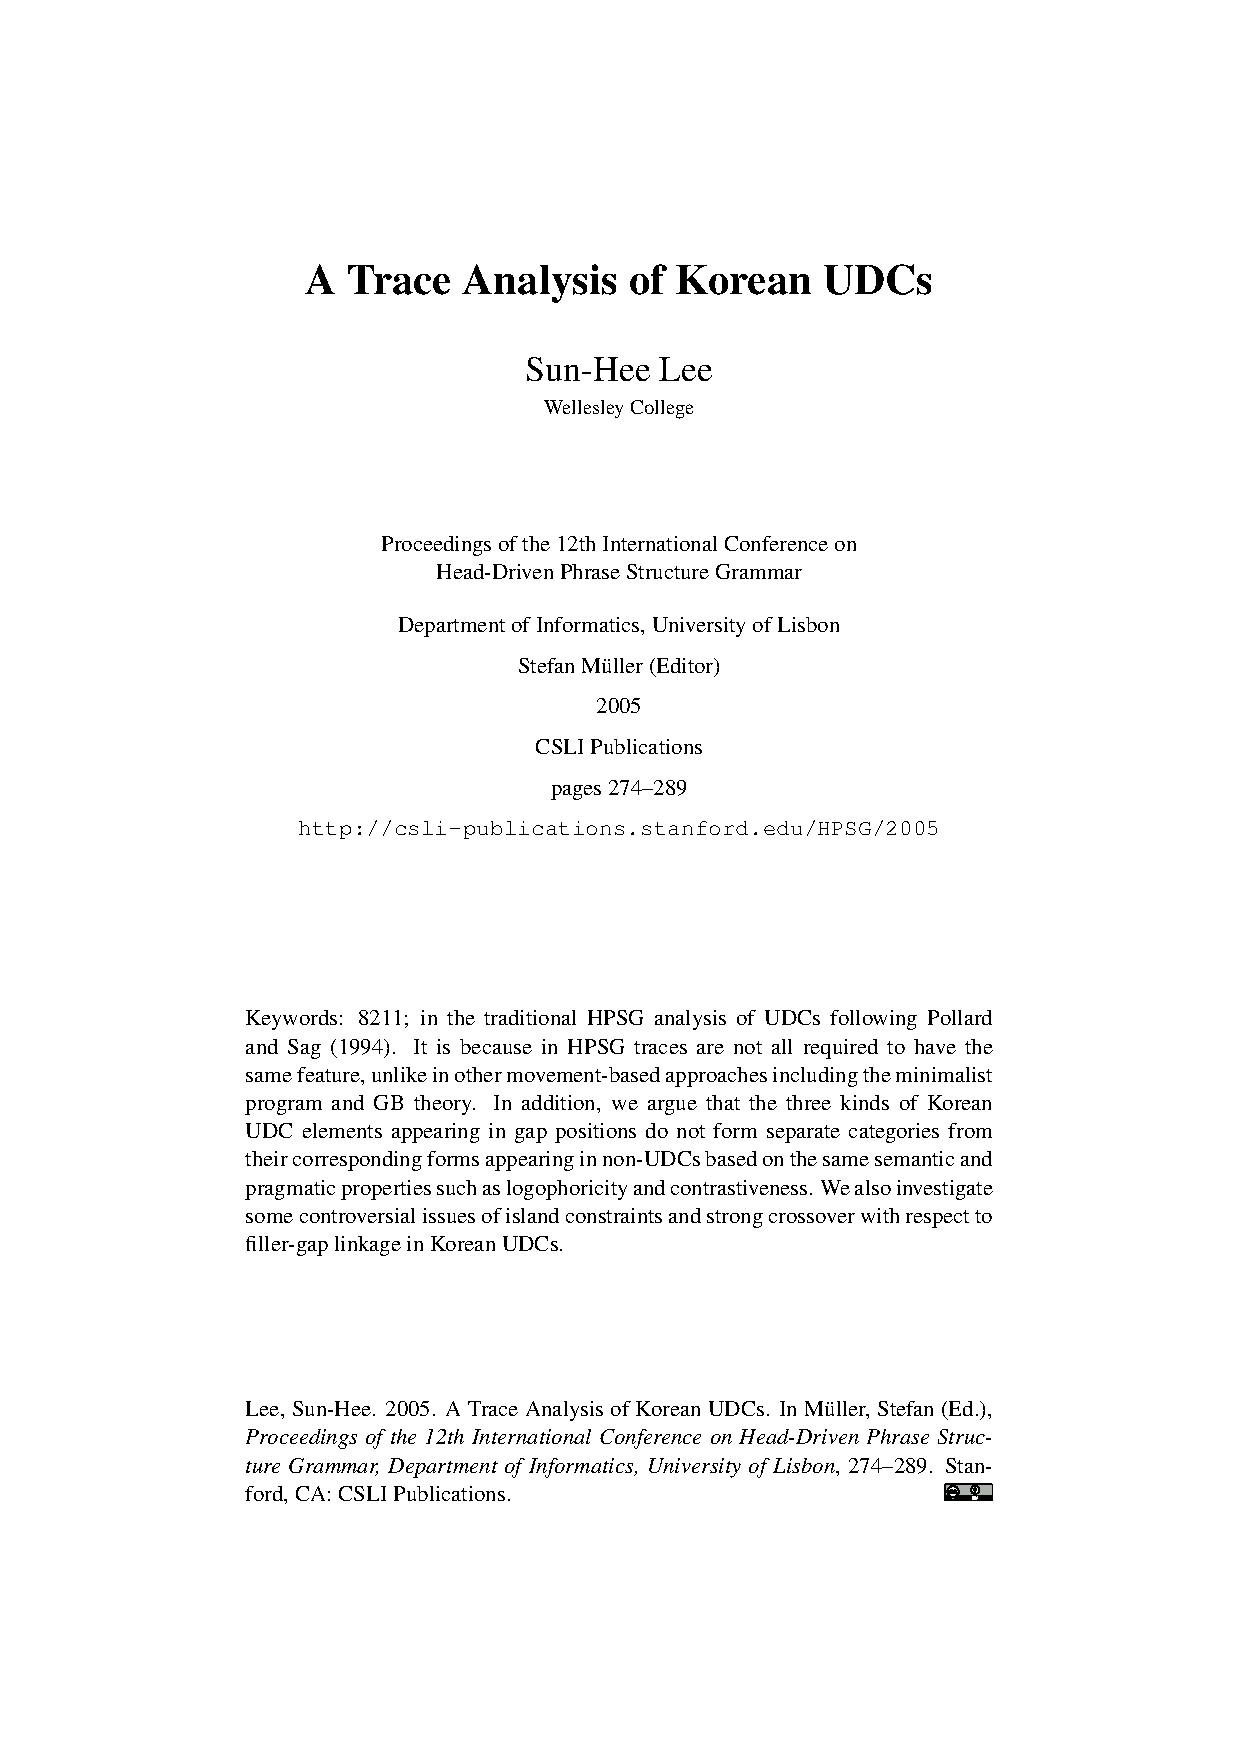
\includepdf[pages=-,pagecommand=\thispagestyle{plain}]{Includes/lee.pdf}
        \end{document}
